\documentclass[12pt,a4paper]{amsart}
\usepackage[utf8]{inputenc}
\usepackage[T1]{fontenc}
\usepackage{amsmath,amsfonts,amssymb}
\usepackage{tikz}
\usepackage{algorithm}
\usepackage{algorithmic}
\usepackage{listings}
\usepackage{xcolor}
\usepackage{geometry}
\usepackage{fancyhdr}
\usepackage{enumitem}
\usepackage{booktabs}
\usepackage{multirow}
\usepackage[hidelinks,bookmarksnumbered,bookmarksopen]{hyperref}
\usepackage{xeCJK}
\setCJKmainfont{LXGW WenKai}

% 页面设置
\geometry{left=2cm,right=2cm,top=2.5cm,bottom=2.5cm}
\pagestyle{fancy}
\fancyhf{}
\fancyhead[L]{查找技术复习总结}
\fancyhead[R]{\thepage}

% TikZ库
\usetikzlibrary{arrows,positioning,shapes,calc,trees,graphs}

% 代码高亮设置
\lstset{
    language=C++,
    basicstyle=\ttfamily\small,
    keywordstyle=\color{blue}\bfseries,
    commentstyle=\color{green!60!black},
    stringstyle=\color{red},
    numbers=left,
    numberstyle=\tiny\color{gray},
    stepnumber=1,
    numbersep=10pt,
    backgroundcolor=\color{gray!10},
    frame=single,
    tabsize=4,
    captionpos=b,
    breaklines=true,
    breakatwhitespace=false,
    showspaces=false,
    showstringspaces=false,
    showtabs=false
}

% 定理环境
\newtheorem{definition}{定义}[section]
\newtheorem{theorem}{定理}[section]
\newtheorem{algorithm_desc}{算法}[section]
\newtheorem{example}{例题}[section]

\title{\textbf{数据结构第七章:查找技术复习总结}}
\author{期末考试复习资料}
\date{\today}

\begin{document}

% \maketitle

% % 目录设置
% \tableofcontents
% \newpage

\section{查找的基本概念}

\subsection{基本术语与定义}

\begin{definition}[记录与关键码]
在查找问题中,通常将数据元素称为\textbf{记录}(record)。可以标识一个记录的某个数据项称为\textbf{关键码}(key),关键码的值称为\textbf{键值}(keyword)。若关键码可以唯一标识一个记录,则称此关键码为\textbf{主关键码}(primary key);反之,称此关键码为\textbf{次关键码}(second key)。
\end{definition}

\begin{center}
\begin{tikzpicture}[scale=1.2]
    % 记录结构示意图
    \node[draw,rectangle,minimum width=6cm,minimum height=0.8cm] (record) at (0,0) {记录};
    \node[draw,rectangle,minimum width=1.2cm,minimum height=0.6cm,fill=red!20] (key) at (-2,-1.2) {关键码};
    \node[draw,rectangle,minimum width=1.2cm,minimum height=0.6cm,fill=blue!20] (data1) at (-0.5,-1.2) {数据1};
    \node[draw,rectangle,minimum width=1.2cm,minimum height=0.6cm,fill=blue!20] (data2) at (1,-1.2) {数据2};
    \node[draw,rectangle,minimum width=1.2cm,minimum height=0.6cm,fill=blue!20] (data3) at (2.5,-1.2) {数据3};
    
    \draw[->] (record.south) -- (key.north);
    \draw[->] (record.south) -- (data1.north);
    \draw[->] (record.south) -- (data2.north);
    \draw[->] (record.south) -- (data3.north);
    
    \node at (0,-2.2) {\textbf{记录结构示意图}};
\end{tikzpicture}
\end{center}

\begin{definition}[查找]
广义地讲,查找(search)是在具有相同类型的记录构成的集合中找出满足给定条件的记录。若在查找集合中找到了与给定值相等的记录,则称\textbf{查找成功};否则称\textbf{查找不成功}(或查找失败)。
\end{definition}

\begin{definition}[静态查找与动态查找]
不涉及插入和删除操作的查找称为\textbf{静态查找}(static search),静态查找在查找不成功时,只返回一个不成功标志,查找的结果不改变查找集合;涉及插入和删除操作的查找称为\textbf{动态查找}(dynamic search),动态查找在查找不成功时,需要将被查找的记录插入到查找集合中。
\end{definition}

\subsection{查找算法的性能分析}

\begin{definition}[平均查找长度]
查找算法的基本操作通常是将记录和给定值进行比较,所以,通常以记录的平均比较次数来度量查找算法的平均时间性能,称为\textbf{平均查找长度}(Average Search Length, ASL)。对于查找成功的情况,其计算公式为:
\begin{equation}
\text{ASL} = \sum_{i=1}^{n} p_i c_i
\end{equation}
其中,$n$为问题规模,查找集合中的记录个数;$p_i$为查找第$i$个记录的概率;$c_i$为查找第$i$个记录所需的比较次数。
\end{definition}

\section{线性表的查找技术}

\subsection{顺序查找}

\begin{definition}[顺序查找]
顺序查找(sequential search)又称线性查找,其基本思想为:从线性表的一端向另一端逐个将记录与给定值进行比较,若相等,则查找成功,给出该记录在表中的位置;若整个表检测完仍未找到与给定值相等的记录,则查找失败。
\end{definition}

\begin{algorithm}
\caption{顺序查找(带哨兵)}
\begin{algorithmic}[1]
\REQUIRE 查找表$data[1..n]$,待查值$k$
\ENSURE 查找成功返回位置,失败返回0
\STATE $i \leftarrow n$ \COMMENT{从表高端开始}
\STATE $data[0] \leftarrow k$ \COMMENT{设置哨兵}
\WHILE{$data[i] \neq k$}
    \STATE $i \leftarrow i - 1$
\ENDWHILE
\RETURN $i$
\end{algorithmic}
\end{algorithm}

\begin{theorem}[顺序查找的性能]
设每个记录的查找概率相等,即$p_i = 1/n \quad (1 \leq i \leq n)$,则:
\begin{itemize}
\item 查找成功时的平均查找长度:
\begin{equation}
\text{ASL}_{\text{成功}} = \frac{1}{n}\sum_{i=1}^{n}(n-i+1) = \frac{n+1}{2} = O(n)
\end{equation}
\item 查找失败时的平均查找长度:
\begin{equation}
\text{ASL}_{\text{失败}} = n+1 = O(n)
\end{equation}
\end{itemize}
\end{theorem}

\subsection{折半查找}

\begin{definition}[折半查找]
折半查找(binary search)的基本思想是:假设有序表按关键码升序排列,取中间记录作为比较对象,若给定值与中间记录相等,则查找成功;若给定值小于中间记录,则在有序表的左半区继续查找;若给定值大于中间记录,则在有序表的右半区继续查找。
\end{definition}

\begin{algorithm}
\caption{折半查找(非递归)}
\begin{algorithmic}[1]
\REQUIRE 有序表$data[1..n]$,待查值$k$
\ENSURE 查找成功返回位置,失败返回0
\STATE $low \leftarrow 1, high \leftarrow n$
\WHILE{$low \leq high$}
    \STATE $mid \leftarrow \lfloor(low + high)/2\rfloor$
    \IF{$k < data[mid]$}
        \STATE $high \leftarrow mid - 1$
    \ELSIF{$k > data[mid]$}
        \STATE $low \leftarrow mid + 1$
    \ELSE
        \RETURN $mid$
    \ENDIF
\ENDWHILE
\RETURN $0$
\end{algorithmic}
\end{algorithm}

\begin{theorem}[折半查找的性能]
设判定树是深度为$k$的满二叉树$(n = 2^k - 1)$,若有序表中每个记录的查找概率相等,即$p_i = 1/n \quad (1 \leq i \leq n)$,则折半查找的平均查找长度为:
\begin{equation}
\text{ASL} = \frac{1}{n}\sum_{j=1}^{k} j \times 2^{j-1} \approx \log_2(n+1) - 1 = O(\log n)
\end{equation}
\end{theorem}

\begin{example}[折半查找过程]
在有序表$\{7,14,18,21,23,29,31,35,38\}$中查找18:
\begin{enumerate}
\item 初始:$low=1, high=9, mid=5$,$data[5]=23 > 18$,令$high=4$
\item $low=1, high=4, mid=2$,$data[2]=14 < 18$,令$low=3$
\item $low=3, high=4, mid=3$,$data[3]=18 = 18$,查找成功
\end{enumerate}
比较次数:3次
\end{example}

\section{树表的查找技术}

\subsection{二叉排序树}

\begin{definition}[二叉排序树]
二叉排序树(Binary Sort Tree, BST)又称二叉查找树,或者是一棵空的二叉树,或者是具有下列性质的二叉树:
\begin{enumerate}
\item 若左子树不空,则左子树上所有结点的值均小于根结点的值;
\item 若右子树不空,则右子树上所有结点的值均大于根结点的值;
\item 左右子树也都是二叉排序树。
\end{enumerate}
\end{definition}

\begin{center}
\begin{tikzpicture}[level distance=1.5cm,
level 1/.style={sibling distance=4cm},
level 2/.style={sibling distance=2cm},
level 3/.style={sibling distance=1.5cm}]
\node [circle,draw] {50}
    child {node [circle,draw] {30}
        child {node [circle,draw] {20}
            child {node [circle,draw] {10}}
            child[missing]}
        child {node [circle,draw] {40}
            child[missing] 
            child {node [circle,draw] {45}}}}
    child {node [circle,draw] {70}
        child {node [circle,draw] {60}}
        child {node [circle,draw] {80}
            child[missing]
            child {node [circle,draw] {90}}}};
\node at (0,-5) {\textbf{二叉排序树示例}};
\end{tikzpicture}
\end{center}

\begin{algorithm}
\caption{二叉排序树查找}
\begin{algorithmic}[1]
\REQUIRE 二叉排序树根结点$T$,待查关键码$k$
\ENSURE 查找成功返回结点指针,失败返回NULL
\IF{$T = NULL$ or $k = T \rightarrow key$}
    \RETURN $T$
\ELSIF{$k < T \rightarrow key$}
    \RETURN BSTSearch($T \rightarrow lchild, k$)
\ELSE
    \RETURN BSTSearch($T \rightarrow rchild, k$)
\ENDIF
\end{algorithmic}
\end{algorithm}

\begin{algorithm}
\caption{二叉排序树插入}
\begin{algorithmic}[1]
\REQUIRE 二叉排序树根结点$T$,待插入关键码$k$
\ENSURE 插入成功返回TRUE,失败返回FALSE
\IF{$T = NULL$}
    \STATE 创建新结点,关键码为$k$
    \RETURN TRUE
\ELSIF{$k = T \rightarrow key$}
    \RETURN FALSE \COMMENT{关键码已存在}
\ELSIF{$k < T \rightarrow key$}
    \RETURN BSTInsert($T \rightarrow lchild, k$)
\ELSE
    \RETURN BSTInsert($T \rightarrow rchild, k$)
\ENDIF
\end{algorithmic}
\end{algorithm}

\begin{theorem}[二叉排序树性能]
二叉排序树查找的时间复杂度:
\begin{itemize}
\item 最好情况(完全二叉树):$O(\log n)$
\item 最坏情况(单支树):$O(n)$
\item 平均情况:$O(\log n)$
\end{itemize}
\end{theorem}

\subsection{平衡二叉树(AVL树)}

\begin{definition}[平衡二叉树]
平衡二叉树(Balanced Binary Tree)或AVL树是一种特殊的二叉排序树,满足:
\begin{enumerate}
\item 是一棵二叉排序树;
\item 对任意结点,其左右子树的高度差的绝对值不超过1。
\end{enumerate}
结点的\textbf{平衡因子}(Balance Factor, BF)定义为该结点左子树的高度减去右子树的高度。AVL树中任一结点的平衡因子只能是-1、0或1。
\end{definition}

\begin{center}
\begin{tikzpicture}[level distance=1.2cm,
level 1/.style={sibling distance=2cm},
level 2/.style={sibling distance=1cm}]
% 失衡情况:LL型
\node at (-6,2) {\textbf{LL型失衡}};
\node[circle,draw,minimum size=8mm] at (-6,0) {$C$}
    child {node[circle,draw,minimum size=8mm] {$B$}
        child {node[circle,draw,minimum size=8mm] {$A$}}
        child[missing]}
    child[missing];
\node at (-6,-2.8) {失衡};

% 调整后
\node at (-2.5,2) {\textbf{右旋调整}};
\node[circle,draw,minimum size=8mm] at (-2.5,0) {$B$}
    child {node[circle,draw,minimum size=8mm] {$A$}}
    child {node[circle,draw,minimum size=8mm] {$C$}};
\node at (-2.5,-2.8) {平衡};

\draw[->,thick] (-4.8,0) -- (-3.2,0);

% 失衡情况:RR型
\node at (1.5,2) {\textbf{RR型失衡}};
\node[circle,draw,minimum size=8mm] at (1.5,0) {$A$}
    child[missing]
    child {node[circle,draw,minimum size=8mm] {$B$}
        child[missing]
        child {node[circle,draw,minimum size=8mm] {$C$}}};
\node at (1.5,-2.8) {失衡};

% 调整后
\node at (5,2) {\textbf{左旋调整}};
\node[circle,draw,minimum size=8mm] at (5,0) {$B$}
    child {node[circle,draw,minimum size=8mm] {$A$}}
    child {node[circle,draw,minimum size=8mm] {$C$}};
\node at (5,-2.8) {平衡};

\draw[->,thick] (3.2,0) -- (3.8,0);
\end{tikzpicture}
\end{center}

\begin{center}
\begin{tikzpicture}[level distance=1.2cm,
level 1/.style={sibling distance=2cm},
level 2/.style={sibling distance=1cm}]
% 失衡情况:LR型
\node at (-3.5,2) {\textbf{LR型失衡}};
\node[circle,draw,minimum size=8mm] at (-3.5,0) {$C$}
    child {node[circle,draw,minimum size=8mm] {$A$}
        child[missing]
        child {node[circle,draw,minimum size=8mm] {$B$}}}
    child[missing];
\node at (-3.5,-2.8) {失衡};

% 调整后
\node at (-0.5,2) {\textbf{左旋-右旋调整}};
\node[circle,draw,minimum size=8mm] at (-0.5,0) {$B$}
    child {node[circle,draw,minimum size=8mm] {$A$}}
    child {node[circle,draw,minimum size=8mm] {$C$}};
\node at (-0.5,-2.8) {平衡};

\draw[->,thick] (-2.3,0) -- (-1.7,0);

% 失衡情况:RL型
\node at (2.5,2) {\textbf{RL型失衡}};
\node[circle,draw,minimum size=8mm] at (2.5,0) {$A$}
    child[missing]
    child {node[circle,draw,minimum size=8mm] {$C$}
        child {node[circle,draw,minimum size=8mm] {$B$}}
        child[missing]};
\node at (2.5,-2.8) {失衡};

% 调整后
\node at (5.5,2) {\textbf{右旋-左旋调整}};
\node[circle,draw,minimum size=8mm] at (5.5,0) {$B$}
    child {node[circle,draw,minimum size=8mm] {$A$}}
    child {node[circle,draw,minimum size=8mm] {$C$}};
\node at (5.5,-2.8) {平衡};

\draw[->,thick] (3.7,0) -- (4.3,0);
\end{tikzpicture}
\end{center}

\begin{example}[平衡二叉树构建示例]
按顺序$\{10,24,32,80,55,30\}$构建平衡二叉树的过程:

给定插入顺序:$\{10, 24, 32, 80, 55, 30\}$

\textbf{步骤1:插入10}
\begin{center}
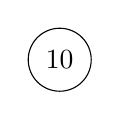
\begin{tikzpicture}[level distance=1.2cm]
\node[circle,draw,minimum size=8mm] {$10$};
\end{tikzpicture}
\end{center}
\begin{center}
根节点:10,平衡因子:0,树平衡
\end{center}

\textbf{步骤2:插入24}
\begin{center}
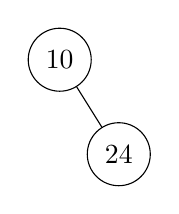
\begin{tikzpicture}[level distance=1.2cm]
\node[circle,draw,minimum size=8mm] {$10$}
    child[missing]
    child {node[circle,draw,minimum size=8mm] {$24$}};
\end{tikzpicture}
\end{center}
\begin{center}
根节点:10,平衡因子:$BF(10) = 0 - 1 = -1$,$BF(24) = 0$,树平衡
\end{center}

\textbf{步骤3:插入32}
\begin{center}
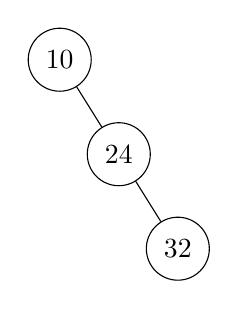
\begin{tikzpicture}[level distance=1.2cm]
\node[circle,draw,minimum size=8mm] {$10$}
    child[missing]
    child {node[circle,draw,minimum size=8mm] {$24$}
        child[missing]
        child {node[circle,draw,minimum size=8mm] {$32$}}};
\end{tikzpicture}
\end{center}
\begin{center}
根节点:10,平衡因子:$BF(10) = 0 - 2 = -2$,$BF(24) = -1$,$BF(32) = 0$
\end{center}
\begin{center}
\textcolor{red}{节点10失衡!RR型不平衡,需要左旋}
\end{center}

\textbf{左旋调整后(以24为轴):}
\begin{center}
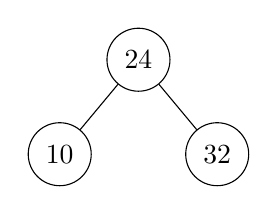
\begin{tikzpicture}[level distance=1.2cm,
level 1/.style={sibling distance=2cm}]
\node[circle,draw,minimum size=8mm] {$24$}
    child {node[circle,draw,minimum size=8mm] {$10$}}
    child {node[circle,draw,minimum size=8mm] {$32$}};
\end{tikzpicture}
\end{center}
\begin{center}
根节点:24,所有节点平衡因子为0,树平衡
\end{center}

\textbf{步骤4:插入80}
\begin{center}
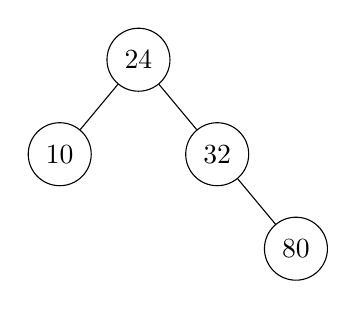
\begin{tikzpicture}[level distance=1.2cm,
level 1/.style={sibling distance=2cm}]
\node[circle,draw,minimum size=8mm] {$24$}
    child {node[circle,draw,minimum size=8mm] {$10$}}
    child {node[circle,draw,minimum size=8mm] {$32$}
        child[missing]
        child {node[circle,draw,minimum size=8mm] {$80$}}};
\end{tikzpicture}
\end{center}
\begin{center}
根节点:24,平衡因子:$BF(24) = 1 - 2 = -1$,$BF(32) = -1$,树平衡
\end{center}

\textbf{步骤5:插入55}
\begin{center}
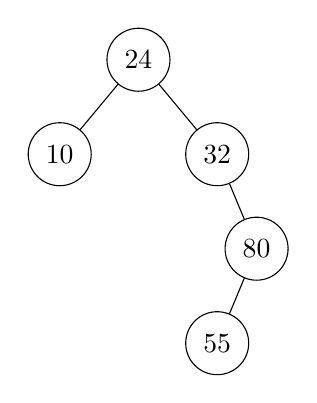
\begin{tikzpicture}[level distance=1.2cm,
level 1/.style={sibling distance=2cm},
level 2/.style={sibling distance=1cm}]
\node[circle,draw,minimum size=8mm] {$24$}
    child {node[circle,draw,minimum size=8mm] {$10$}}
    child {node[circle,draw,minimum size=8mm] {$32$}
        child[missing]
        child {node[circle,draw,minimum size=8mm] {$80$}
            child {node[circle,draw,minimum size=8mm] {$55$}}
            child[missing]}};
\end{tikzpicture}
\end{center}
\begin{center}
根节点:24,平衡因子:$BF(32) = 0 - 2 = -2$,$BF(80) = 1$
\end{center}
\begin{center}
\textcolor{red}{节点32失衡!RL型不平衡,需要RL旋转}
\end{center}

\textbf{RL型调整:对80先右旋,再对32左旋}
\begin{center}
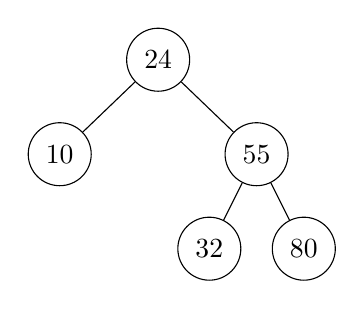
\begin{tikzpicture}[level distance=1.2cm,
level 1/.style={sibling distance=2.5cm},
level 2/.style={sibling distance=1.2cm}]
\node[circle,draw,minimum size=8mm] {$24$}
    child {node[circle,draw,minimum size=8mm] {$10$}}
    child {node[circle,draw,minimum size=8mm] {$55$}
        child {node[circle,draw,minimum size=8mm] {$32$}}
        child {node[circle,draw,minimum size=8mm] {$80$}}};
\end{tikzpicture}
\end{center}
\begin{center}
根节点:24,所有节点平衡,树平衡
\end{center}

\textbf{步骤6:插入30}
\begin{center}
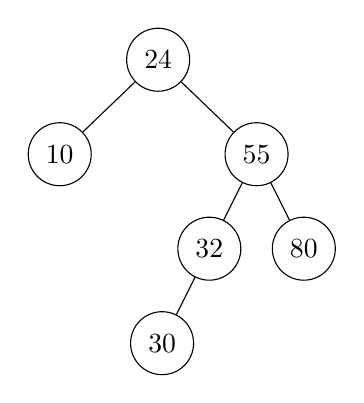
\begin{tikzpicture}[level distance=1.2cm,
level 1/.style={sibling distance=2.5cm},
level 2/.style={sibling distance=1.2cm}]
\node[circle,draw,minimum size=8mm] {$24$}
    child {node[circle,draw,minimum size=8mm] {$10$}}
    child {node[circle,draw,minimum size=8mm] {$55$}
        child {node[circle,draw,minimum size=8mm] {$32$}
            child {node[circle,draw,minimum size=8mm] {$30$}}
            child[missing]}
        child {node[circle,draw,minimum size=8mm] {$80$}}};
\end{tikzpicture}
\end{center}
\begin{center}
根节点:24,平衡因子:$BF(24) = 1 - 3 = -2$,$BF(55) = 2 - 1 = 1$,$BF(32) = 1$
\end{center}
\begin{center}
\textcolor{red}{节点24失衡!需要左旋调整}
\end{center}

\textbf{左旋调整过程:以55为新根}
\begin{center}
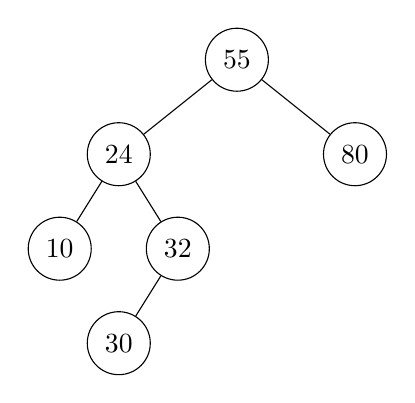
\begin{tikzpicture}[level distance=1.2cm,
level 1/.style={sibling distance=3cm},
level 2/.style={sibling distance=1.5cm}]
\node[circle,draw,minimum size=8mm] {$55$}
    child {node[circle,draw,minimum size=8mm] {$24$}
        child {node[circle,draw,minimum size=8mm] {$10$}}
        child {node[circle,draw,minimum size=8mm] {$32$}
            child {node[circle,draw,minimum size=8mm] {$30$}}
            child[missing]}}
    child {node[circle,draw,minimum size=8mm] {$80$}};
\end{tikzpicture}
\end{center}
\begin{center}
根节点:55,所有节点平衡因子在[-1,1]范围内,树平衡
\end{center}

等等,让我重新分析步骤6的旋转。实际上应该进行如下操作:

\textbf{重新分析步骤6:插入30后的调整}
插入30后,节点24的平衡因子变为-2,这是一个复杂的情况。路径是24→55→32→30,这构成RL型不平衡。

\textbf{正确的RL型调整:}
\begin{enumerate}
\item 先对55的左子树32进行右旋
\item 再对24进行左旋,以调整后的节点为轴
\end{enumerate}

经过正确的RL旋转后:
\begin{center}
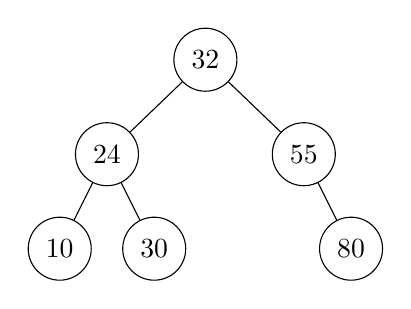
\begin{tikzpicture}[level distance=1.2cm,
level 1/.style={sibling distance=2.5cm},
level 2/.style={sibling distance=1.2cm}]
\node[circle,draw,minimum size=8mm] {$32$}
    child {node[circle,draw,minimum size=8mm] {$24$}
        child {node[circle,draw,minimum size=8mm] {$10$}}
        child {node[circle,draw,minimum size=8mm] {$30$}}}
    child {node[circle,draw,minimum size=8mm] {$55$}
        child[missing]
        child {node[circle,draw,minimum size=8mm] {$80$}}};
\end{tikzpicture}
\end{center}

\textbf{最终的平衡二叉树:}
\begin{center}
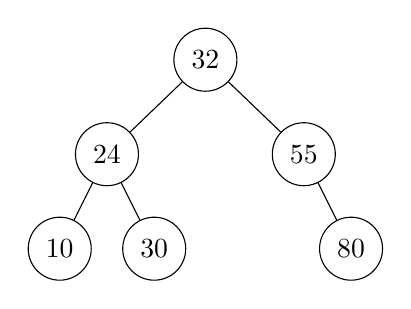
\begin{tikzpicture}[level distance=1.2cm,
level 1/.style={sibling distance=2.5cm},
level 2/.style={sibling distance=1.2cm}]
\node[circle,draw,minimum size=8mm] {$32$}
    child {node[circle,draw,minimum size=8mm] {$24$}
        child {node[circle,draw,minimum size=8mm] {$10$}}
        child {node[circle,draw,minimum size=8mm] {$30$}}}
    child {node[circle,draw,minimum size=8mm] {$55$}
        child[missing]
        child {node[circle,draw,minimum size=8mm] {$80$}}};
\end{tikzpicture}
\end{center}
\begin{center}
\textcolor{green}{最终根节点为32,所有节点都平衡!}
\end{center}

\textbf{答案:B. 32}

\textbf{解释:}在平衡二叉树的构建过程中,通过一系列的旋转操作来维持树的平衡性。最终构建完成的平衡二叉树的根节点是32。
\end{example}


\subsection{B树}

\begin{definition}[m阶B树]
一棵m阶B树(B-tree)或为空树,或为满足下列性质的m叉树:
\begin{enumerate}
\item 树中每个结点最多含有$m$个孩子($m \geq 2$);
\item 若根结点不是叶子结点,则至少有2个孩子;
\item 除根结点和叶子结点外,其它每个结点至少有$\lceil m/2 \rceil$个孩子;
\item 所有叶子结点出现在同一层,叶子结点不包含任何信息;
\item 有$k$个孩子的非叶子结点有$k-1$个关键码,关键码按升序排列。
\end{enumerate}
\end{definition}

\begin{center}
\begin{tikzpicture}[level distance=2cm,
level 1/.style={sibling distance=6cm},
level 2/.style={sibling distance=2cm}]
% 3阶B树示例
\node[rectangle,draw,minimum width=2cm] {$20 \mid 50$}
    child {node[rectangle,draw,minimum width=1.5cm] {$10$}
        child {node[rectangle,draw,minimum width=0.8cm] {$5$}}
        child {node[rectangle,draw,minimum width=0.8cm] {$15$}}}
    child {node[rectangle,draw,minimum width=1.5cm] {$30 \mid 40$}
        child {node[rectangle,draw,minimum width=0.8cm] {$25$}}
        child {node[rectangle,draw,minimum width=0.8cm] {$35$}}
        child {node[rectangle,draw,minimum width=0.8cm] {$45$}}}
    child {node[rectangle,draw,minimum width=1.5cm] {$60 \mid 70$}
        child {node[rectangle,draw,minimum width=0.8cm] {$55$}}
        child {node[rectangle,draw,minimum width=0.8cm] {$65$}}
        child {node[rectangle,draw,minimum width=0.8cm] {$75$}}};
\node at (0,-4.5) {\textbf{3阶B树示例}};
\end{tikzpicture}
\end{center}

\section{散列表查找技术}

\subsection{散列表的基本概念}

\begin{definition}[散列表]
散列表(Hash Table)又称哈希表,是根据关键码值直接进行访问的数据结构。通过把关键码值映射到表中一个位置来访问记录,以加快查找的速度。这个映射函数叫做\textbf{散列函数}(Hash Function),存放记录的数组叫做\textbf{散列表}。
\end{definition}

\begin{definition}[散列冲突]
对不同的关键码$k_i \neq k_j$,有$H(k_i) = H(k_j)$,这种现象称为\textbf{冲突}(collision)或\textbf{碰撞}。具有相同函数值的关键码对该散列函数来说称作\textbf{同义词}。
\end{definition}

\subsection{散列函数构造}

\begin{theorem}[除留余数法]
设散列表表长为$m$,取一个不大于$m$的质数$p$,散列函数为:
\begin{equation}
H(key) = key \bmod p
\end{equation}
其中$p$最好选择接近$m$的质数。
\end{theorem}

\begin{theorem}[数字分析法]
设关键码是$r$进制数,而$r$个数码在各位上出现的频率不一定相同,可能在某些位上分布比较均匀,每种数码出现的机会大致相等,在某些位上分布不均匀,只有某几种数码经常出现。此时应选取数码分布较为均匀的若干位作为散列地址。
\end{theorem}

\subsection{处理冲突的方法}

\begin{definition}[开放定址法]
开放定址法的一般形式为:
$$H_i = (H(key) + d_i) \bmod m \quad (i = 0,1,2,\ldots,k(k \leq m-1))$$
其中$H(key)$为散列函数;$d_i$为增量序列;$m$为散列表表长。
\begin{itemize}
\item \textbf{线性探测再散列}:$d_i = 0,1,2,3,\ldots,m-1$
\item \textbf{二次探测再散列}:$d_i = 0^2, 1^2, -1^2, 2^2, -2^2, \ldots, \pm k^2$
\item \textbf{伪随机探测再散列}:$d_i$为伪随机数序列
\end{itemize}
\end{definition}

\begin{definition}[链地址法]
将所有关键码为同义词的记录存储在同一线性链表中。设散列地址为$i$的同义词链表的头指针存放在散列表的第$i$个单元中,因而查找、插入和删除主要在同义词链中进行。
\end{definition}

\begin{center}
\begin{tikzpicture}[scale=1]
% 散列表
\foreach \i in {0,...,6} {
    \node[draw,rectangle,minimum width=1cm,minimum height=0.63cm] (hash\i) at (0,-\i*0.8) {\i};
}

% 链表节点和连接
% 第一行链表 (hash1): 10 -> 24 -> null
\node[draw,circle] (node10) at (2,-0.8) {10};
\node[draw,circle] (node24) at (3.5,-0.8) {24};
\draw[->] (hash1) -- (node10);
\draw[->] (node10) -- (node24);
\draw[->] (node24) -- (5,-0.8) node[right] {$\phi$};

% 第二行链表 (hash2): 23 -> 16 -> null
\node[draw,circle] (node23) at (2,-1.6) {23};
\node[draw,circle] (node16) at (3.5,-1.6) {16};
\draw[->] (hash2) -- (node23);
\draw[->] (node23) -- (node16);
\draw[->] (node16) -- (5,-1.6) node[right] {$\phi$};

% 第三行链表 (hash4): 17 -> null
\node[draw,circle] (node17) at (2,-3.2) {17};
\draw[->] (hash4) -- (node17);
\draw[->] (node17) -- (3.5,-3.2) node[right] {$\phi$};

\node at (2.5,-5.5) {\textbf{链地址法处理冲突}};
\end{tikzpicture}
\end{center}




\section{各种查找方法的比较}

\begin{center}
\begin{tabular}{|l|c|c|c|c|}
\hline
\textbf{查找方法} & \textbf{平均时间复杂度} & \textbf{最坏时间复杂度} & \textbf{空间复杂度} & \textbf{是否有序} \\
\hline
顺序查找 & $O(n)$ & $O(n)$ & $O(1)$ & 否 \\
\hline
折半查找 & $O(\log n)$ & $O(\log n)$ & $O(1)$ & 是 \\
\hline
二叉排序树 & $O(\log n)$ & $O(n)$ & $O(n)$ & 否 \\
\hline
平衡二叉树 & $O(\log n)$ & $O(\log n)$ & $O(n)$ & 否 \\
\hline
B树 & $O(\log n)$ & $O(\log n)$ & $O(n)$ & 是 \\
\hline
散列表 & $O(1)$ & $O(n)$ & $O(n)$ & 否 \\
\hline
\end{tabular}
\end{center}

\section{典型例题分析}

\begin{example}[折半查找过程分析]
在有序表$(3,8,12,15,27,33,48,66,75,87,96)$中查找关键码48,写出每步比较过程,并计算比较次数。

\textbf{解:}
\begin{enumerate}
\item 初始:$low=1, high=11, mid=6$,$a[6]=33 < 48$,$low=7$
\item $low=7, high=11, mid=9$,$a[9]=75 > 48$,$high=8$  
\item $low=7, high=8, mid=7$,$a[7]=48 = 48$,查找成功
\end{enumerate}
比较次数:3次
\end{example}

\begin{example}[二叉排序树构造]
根据关键码序列$(45,24,53,12,37,93,67)$构造二叉排序树。

\textbf{解:}
\begin{center}
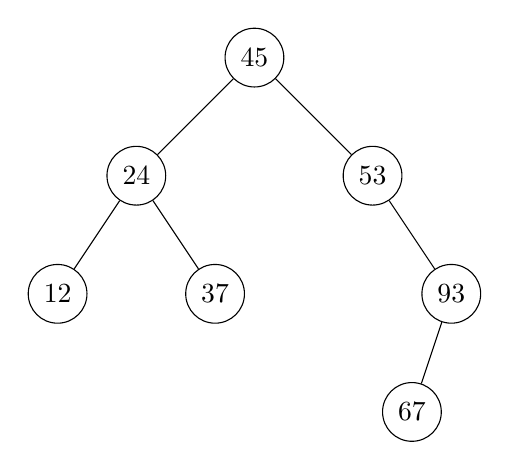
\begin{tikzpicture}[level distance=1.5cm,
level 1/.style={sibling distance=3cm},
level 2/.style={sibling distance=2cm},
level 3/.style={sibling distance=1cm}]
\node [circle,draw] {45}
    child {node [circle,draw] {24}
        child {node [circle,draw] {12}}
        child {node [circle,draw] {37}}}
    child {node [circle,draw] {53}
        child[missing]
        child {node [circle,draw] {93}
            child {node [circle,draw] {67}}
            child[missing]}};
\end{tikzpicture}
\end{center}
插入过程:
\begin{enumerate}
\item 插入45:作为根结点
\item 插入24:$24 < 45$,作为45的左孩子
\item 插入53:$53 > 45$,作为45的右孩子
\item 插入12:$12 < 45, 12 < 24$,作为24的左孩子
\item 插入37:$37 < 45, 37 > 24$,作为24的右孩子
\item 插入93:$93 > 45, 93 > 53$,作为53的右孩子  
\item 插入67:$67 > 45, 67 > 53, 67 < 93$,作为93的左孩子
\end{enumerate}
\end{example}

\begin{example}[散列表构造]
设散列函数$H(k) = k \bmod 13$,用线性探测再散列法解决冲突,将关键码序列$(19,14,23,01,68,20,84,27,55,11,10,79)$存入散列表。

\textbf{解:}
\begin{center}
\begin{tabular}{|c|c|c|c|c|c|c|c|c|c|c|c|c|c|}
\hline
地址 & 0 & 1 & 2 & 3 & 4 & 5 & 6 & 7 & 8 & 9 & 10 & 11 & 12 \\
\hline
关键码 & & 01 & 14 & 27 & 68 & 55 & 19 & 20 & 84 & 23 & 10 & 11 & 79 \\
\hline
\end{tabular}
\end{center}

插入过程分析:
\begin{itemize}
\item $H(19) = 6$,散列到地址6
\item $H(14) = 1$,散列到地址1  
\item $H(23) = 10$,地址10被占用,探测到地址9
\item $H(01) = 1$,地址1空闲,散列到地址1
\item $\ldots$
\end{itemize}
\end{example}

\section{扩展知识}

\subsection{分块查找}

\begin{definition}[分块查找]
分块查找又称索引顺序查找,是顺序查找的改进方法。基本思想是将查找表分为若干子块,块内的记录可以无序,但块间必须有序,即第一个块中的最大关键码小于第二个块中的所有记录的关键码,第二个块中的最大关键码小于第三个块中的所有记录的关键码,以此类推。
\end{definition}

\subsection{B+树}

\begin{definition}[B+树]
B+树是B树的变形,其定义基本与B树相同,区别在于:
\begin{enumerate}
\item 非叶结点仅含有其子树根结点的最大(或最小)关键码;
\item 叶结点包含了全部关键码和相应记录的存储地址,且叶结点按关键码大小顺序链接;
\item 非叶结点相当于叶结点的索引,叶结点相当于存储关键码的数据层。
\end{enumerate}
\end{definition}

\section{复习要点总结}

\subsection{重点掌握内容}
\begin{enumerate}
\item 理解查找的基本概念:平均查找长度ASL的计算
\item 掌握线性表查找:顺序查找、折半查找的算法实现和性能分析
\item 掌握二叉排序树:构造、查找、插入、删除操作
\item 理解平衡二叉树:平衡因子、四种失衡类型及调整方法
\item 掌握散列表:散列函数构造、冲突处理方法
\item 了解B树的基本概念和操作
\end{enumerate}

\subsection{常见考试题型}
\begin{enumerate}
\item ASL计算题
\item 折半查找过程模拟
\item 二叉排序树的构造和操作
\item AVL树的调整过程
\item 散列表的构造和查找过程
\item 各种查找方法的性能比较
\end{enumerate}

\subsection{学习建议}
\begin{enumerate}
\item 熟练掌握各种查找算法的基本思想和实现步骤
\item 重点理解时间复杂度的分析方法
\item 多做练习题,特别是算法模拟题
\item 注意各种数据结构的适用场景和优缺点比较
\end{enumerate}

\end{document}
\end{enumerate}
\end{definition}

\begin{theorem}[二叉排序树的中序遍历性质]
对二叉排序树进行中序遍历可以得到一个有序序列。
\end{theorem}

\subsubsection{二叉排序树的查找}

\begin{algorithm}
\caption{二叉排序树查找(递归)}
\begin{algorithmic}[1]
\REQUIRE 二叉排序树$T$,待查值$k$
\ENSURE 查找成功返回结点指针,失败返回NULL
\IF{$T = \text{NULL}$}
    \RETURN NULL
\ELSIF{$k = T \rightarrow data$}
    \RETURN $T$
\ELSIF{$k < T \rightarrow data$}
    \RETURN SearchBST($T \rightarrow lchild, k$)
\ELSE
    \RETURN SearchBST($T \rightarrow rchild, k$)
\ENDIF
\end{algorithmic}
\end{algorithm}

\subsubsection{二叉排序树的插入}

\begin{algorithm}
\caption{二叉排序树插入}
\begin{algorithmic}[1]
\REQUIRE 二叉排序树$T$,插入值$x$
\ENSURE 返回插入后的树
\IF{$T = \text{NULL}$}
    \STATE 创建新结点$s$,$s \rightarrow data = x$
    \STATE $s \rightarrow lchild = s \rightarrow rchild = \text{NULL}$
    \RETURN $s$
\ELSIF{$T \rightarrow data > x$}
    \STATE $T \rightarrow lchild = \text{InsertBST}(T \rightarrow lchild, x)$
\ELSE
    \STATE $T \rightarrow rchild = \text{InsertBST}(T \rightarrow rchild, x)$
\ENDIF
\RETURN $T$
\end{algorithmic}
\end{algorithm}

\subsubsection{二叉排序树的删除}

删除操作比插入操作复杂,需要考虑三种情况:

\begin{enumerate}
\item \textbf{删除叶子结点}:直接删除,将其双亲结点的相应指针域改为空。
\item \textbf{删除只有一个子树的结点}:用其子树替换该结点。
\item \textbf{删除有两个子树的结点}:用其中序后继(右子树中最小值结点)替换该结点的值,然后删除中序后继结点。
\end{enumerate}

\begin{theorem}[二叉排序树的性能]
二叉排序树的查找、插入、删除操作的时间复杂度:
\begin{itemize}
\item 最好情况(平衡树):$O(\log n)$
\item 最坏情况(退化为单链表):$O(n)$
\item 平均情况:$O(\log n)$
\end{itemize}
\end{theorem}

\subsection{平衡二叉树}

\begin{definition}[平衡二叉树]
平衡二叉树(AVL树)或者是一棵空的二叉排序树,或者是具有下列性质的二叉排序树:
\begin{enumerate}
\item 根结点的左子树和右子树的深度最多相差1;
\item 根结点的左子树和右子树都是平衡二叉树。
\end{enumerate}
\end{definition}

\begin{definition}[平衡因子]
结点的\textbf{平衡因子}(Balance Factor)是该结点的左子树的深度与右子树的深度之差。在平衡二叉树中,结点的平衡因子只可能是$-1, 0, 1$。
\end{definition}

\subsubsection{平衡二叉树的调整}

当插入新结点导致某结点的平衡因子绝对值大于1时,需要进行调整。设$A$为最小不平衡子树的根结点,调整有四种类型:

\begin{enumerate}
\item \textbf{LL型调整}:新结点插在$A$的左孩子的左子树上
\begin{itemize}
\item 操作:对$A$进行右旋转
\item 调整后:$A$的左孩子成为新的根,$A$成为其右孩子
\end{itemize}

\item \textbf{RR型调整}:新结点插在$A$的右孩子的右子树上
\begin{itemize}
\item 操作:对$A$进行左旋转
\item 调整后:$A$的右孩子成为新的根,$A$成为其左孩子
\end{itemize}

\item \textbf{LR型调整}:新结点插在$A$的左孩子的右子树上
\begin{itemize}
\item 操作:先对$A$的左孩子进行左旋转,再对$A$进行右旋转
\end{itemize}

\item \textbf{RL型调整}:新结点插在$A$的右孩子的左子树上
\begin{itemize}
\item 操作:先对$A$的右孩子进行右旋转,再对$A$进行左旋转
\end{itemize}
\end{enumerate}

\begin{theorem}[平衡二叉树的性能]
设$N_h$表示深度为$h$的平衡二叉树中的最少结点个数,则有:
\begin{equation}
N_0 = 0, \quad N_1 = 1, \quad N_h = N_{h-1} + N_{h-2} + 1
\end{equation}
具有$n$个结点的平衡二叉树的深度为$1.44\log_2(n+2) - 1.328$,查找的时间复杂度为$O(\log n)$。
\end{theorem}

\subsection{B树}

\begin{definition}[m阶B树]
一棵$m$阶的B树或者为空树,或者为满足下列特性的$m$叉树:
\begin{enumerate}
\item 每个结点至多有$m$棵子树。
\item 根结点至少有两棵子树。
\item 除根结点外,其他结点至少有$\lceil m/2 \rceil$棵子树。
\item 所有结点包含数据:$(n, A_0, K_1, A_1, K_2, \ldots, K_n, A_n)$,\\
      其中$n(\lceil m/2 \rceil - 1 \leq n \leq m-1)$为关键码个数,\\
      $K_i(1 \leq i \leq n)$为关键码且$K_i < K_{i+1}$,\\
      $A_i(0 \leq i \leq n)$为指向子树根结点的指针。
\item 所有叶子结点都出现在同一层。
\end{enumerate}
\end{definition}

\subsubsection{B树的查找}

B树的查找类似于二叉排序树,但每个结点是多关键码的有序表:
\begin{enumerate}
\item 在结点内进行查找(可用折半查找)
\item 若找到,查找成功
\item 否则,根据比较结果确定下一个要查找的子树
\item 重复上述过程,直到找到或到达外部结点
\end{enumerate}

\begin{theorem}[B树查找的性能]
含有$n$个关键码的$m$阶B树的最大深度是:
\begin{equation}
\log_{\lceil m/2 \rceil}\left(\frac{n+1}{2}\right) + 1
\end{equation}
\end{theorem}

\subsubsection{B树的插入}

B树插入过程:
\begin{enumerate}
\item \textbf{定位}:找到应插入的叶子结点
\item \textbf{插入}:若结点关键码个数小于$m-1$,直接插入
\item \textbf{分裂}:若结点溢出,分裂成两个结点,中间关键码上升到父结点
\item \textbf{递归处理}:若父结点也溢出,继续分裂过程
\end{enumerate}

\subsubsection{B树的删除}

B树删除过程:
\begin{enumerate}
\item \textbf{定位}:找到要删除的关键码
\item \textbf{替换}:若在非叶子结点,用后继关键码替换
\item \textbf{删除}:在叶子结点删除关键码
\item \textbf{调整}:若结点关键码个数少于$\lceil m/2 \rceil - 1$:
\begin{itemize}
\item 借关键码:从兄弟结点借关键码
\item 合并结点:与兄弟结点合并,父结点关键码下移
\end{itemize}
\end{enumerate}

\section{散列表的查找技术}

\subsection{散列查找的基本思想}

\begin{definition}[散列技术]
散列技术是建立记录的存储位置和它的关键码之间的确定对应关系$H$,使得每个关键码$key$和唯一的存储位置$H(key)$相对应。采用散列技术将记录存储在一块连续的存储空间中,这块连续的存储空间称为\textbf{散列表}(hash table)。
\end{definition}

\begin{definition}[散列函数]
将关键码映射为散列表中适当存储位置的函数称为\textbf{散列函数}(hash function),所得的存储位置称为\textbf{散列地址}(hash address)。
\end{definition}

\begin{definition}[冲突]
对于两个不同的关键码$k_1 \neq k_2$,有$H(k_1) = H(k_2)$,即两个不同的记录需要存放在同一个存储位置中,这种现象称为\textbf{冲突}(collision),$k_1$和$k_2$称为\textbf{同义词}(synonym)。
\end{definition}

\subsection{散列函数的设计}

散列函数设计的基本原则:
\begin{enumerate}
\item \textbf{计算简单}:散列函数不应该有很大的计算量
\item \textbf{分布均匀}:散列函数应该把记录以相同概率散列到所有地址空间
\end{enumerate}

\subsubsection{常用散列函数}

\begin{enumerate}
\item \textbf{直接定址法}
\begin{equation}
H(key) = a \times key + b \quad (a, b \text{为常数})
\end{equation}
特点:不会产生冲突,但适用范围有限。

\item \textbf{除留余数法}
\begin{equation}
H(key) = key \bmod p
\end{equation}
其中$p$通常选择小于或等于表长的最小素数。

\item \textbf{平方取中法}
对关键码平方后,按散列表大小,取中间的若干位作为散列地址。
\end{enumerate}

\subsection{处理冲突的方法}

\subsubsection{开放定址法(闭散列表)}

\begin{definition}[开放定址法]
当关键码$key$的散列地址$H(key)$产生冲突时,根据下式寻找下一个空的散列地址:
\begin{equation}
(H(key) + d_i) \bmod m
\end{equation}
\end{definition}

常用的开放定址法:
\begin{enumerate}
\item \textbf{线性探测法}:$d_i = 1, 2, \ldots, m-1$
\item \textbf{二次探测法}:$d_i = 1^2, -1^2, 2^2, -2^2, \ldots, q^2, -q^2$,$q \leq \sqrt{m}$
\end{enumerate}

\begin{remark}[堆积现象]
线性探测法容易产生\textbf{堆积}(clustering)现象,即非同义词之间对同一散列地址的争夺,这会降低查找效率。
\end{remark}

\subsubsection{拉链法(开散列表)}

\begin{definition}[拉链法]
将所有散列地址相同的记录(同义词)存储在一个单链表中,在散列表中存储所有同义词子表的头指针。
\end{definition}

拉链法的特点:
\begin{itemize}
\item 优点:不产生堆积现象,删除操作简单
\item 缺点:需要额外的指针存储空间
\item 平均链长:$n/m$($n$为记录数,$m$为表长)
\end{itemize}

\subsection{散列查找的性能分析}

\begin{definition}[装填因子]
设填入散列表中的记录个数为$n$,散列表的长度为$m$,则\textbf{装填因子}为:
\begin{equation}
\alpha = \frac{n}{m}
\end{equation}
\end{definition}

\begin{theorem}[不同冲突处理方法的平均查找长度]
\begin{center}
\begin{tabular}{|c|c|c|}
\hline
处理冲突方法 & 查找成功时ASL & 查找失败时ASL \\
\hline
线性探测法 & $\frac{1}{2}\left(1+\frac{1}{1-\alpha}\right)$ & $\frac{1}{2}\left(1+\frac{1}{(1-\alpha)^2}\right)$ \\
\hline
二次探测法 & $-\frac{1}{\alpha}\ln(1-\alpha)$ & $\frac{1}{1-\alpha}$ \\
\hline
拉链法 & $1+\frac{\alpha}{2}$ & $\alpha + e^{-\alpha}$ \\
\hline
\end{tabular}
\end{center}
\end{theorem}

\begin{theorem}[散列查找的时间复杂度]
散列表的平均查找长度是装填因子$\alpha$的函数,而不是记录个数$n$的函数。通过选择合适的装填因子,可以将平均查找长度限定在一个范围内,因此散列查找的时间复杂度为$O(1)$。
\end{theorem}

\section{典型例题解析}

\begin{example}[折半查找判定树]
构造长度为7的折半查找判定树,并计算平均查找长度。

\textbf{解:}设有序表为$\{a_1, a_2, a_3, a_4, a_5, a_6, a_7\}$

判定树构造过程:
\begin{enumerate}
\item 根结点:$mid = (1+7)/2 = 4$,选择$a_4$
\item 左子树:对应$\{a_1, a_2, a_3\}$,根为$a_2$
\item 右子树:对应$\{a_5, a_6, a_7\}$,根为$a_6$
\end{enumerate}

各结点的比较次数:
\begin{itemize}
\item 第1层:$a_4$(1次)
\item 第2层:$a_2, a_6$(2次)
\item 第3层:$a_1, a_3, a_5, a_7$(3次)
\end{itemize}

平均查找长度:
\begin{equation}
ASL = \frac{1 \times 1 + 2 \times 2 + 4 \times 3}{7} = \frac{17}{7} \approx 2.43
\end{equation}
\end{example}

\begin{example}[平衡二叉树调整]
向平衡二叉树中依次插入关键码序列$\{20, 35, 40, 15, 30, 25\}$,展示调整过程。

\textbf{解:}
\begin{enumerate}
\item 插入20, 35:形成平衡树
\item 插入40:导致以20为根的子树失衡(RR型),进行左旋转,35成为新根
\item 插入15, 30:保持平衡
\item 插入25:导致以35为根的左子树失衡(LR型),需要双旋转
\begin{itemize}
\item 第一次:对20的右子树以30为轴左旋
\item 第二次:对35以30为轴右旋
\end{itemize}
\end{enumerate}

最终得到以30为根的平衡二叉树。
\end{example}

\begin{example}[散列表构造]
关键码集合$\{47, 7, 29, 11, 16, 92, 22, 8, 3\}$,散列函数$H(key) = key \bmod 11$,分别用线性探测法和拉链法处理冲突。

\textbf{解:}

\textbf{线性探测法:}
\begin{center}
\begin{tabular}{|c|c|c|c|c|c|c|c|c|c|c|c|}
\hline
地址 & 0 & 1 & 2 & 3 & 4 & 5 & 6 & 7 & 8 & 9 & 10 \\
\hline
关键码 & 11 & 22 & & 47 & 92 & 16 & 3 & 7 & 29 & 8 & \\
\hline
\end{tabular}
\end{center}

$ASL_{成功} = \frac{5 \times 1 + 3 \times 2 + 1 \times 4}{9} = \frac{15}{9} \approx 1.67$

\textbf{拉链法:}
同义词链表:
\begin{itemize}
\item $H(key) = 0$: $11$
\item $H(key) = 3$: $47$
\item $H(key) = 5$: $16$
\item $H(key) = 7$: $7 \rightarrow 29$
\item $H(key) = 8$: $8$
\item $H(key) = 9$: $92$
\item $H(key) = 10$: $22 \rightarrow 3$
\end{itemize}

$ASL_{成功} = \frac{6 \times 1 + 3 \times 2}{9} = \frac{12}{9} \approx 1.33$
\end{example}

\section{各种查找方法比较}

\begin{center}
\begin{tabular}{|l|c|c|c|c|}
\hline
\textbf{查找方法} & \textbf{平均时间复杂度} & \textbf{最坏时间复杂度} & \textbf{空间复杂度} & \textbf{适用条件} \\
\hline
顺序查找 & $O(n)$ & $O(n)$ & $O(1)$ & 无序/有序表 \\
\hline
折半查找 & $O(\log n)$ & $O(\log n)$ & $O(1)$ & 有序顺序表 \\
\hline
二叉排序树 & $O(\log n)$ & $O(n)$ & $O(n)$ & 动态查找 \\
\hline
平衡二叉树 & $O(\log n)$ & $O(\log n)$ & $O(n)$ & 动态查找 \\
\hline
B树 & $O(\log n)$ & $O(\log n)$ & $O(n)$ & 外存查找 \\
\hline
散列查找 & $O(1)$ & $O(n)$ & $O(n)$ & 快速查找 \\
\hline
\end{tabular}
\end{center}

\section{扩展知识}

\subsection{分块查找}

\begin{definition}[分块查找]
分块查找又称索引顺序查找,将线性表分为若干块,块间有序,块内无序。建立索引表记录每块的最大关键码和块首地址。查找分两步:先在索引表中确定块,再在块内顺序查找。
\end{definition}

设$n$个记录分为$m$个块,每块$t$个记录($n = m \times t$),则:
\begin{equation}
ASL = \frac{m+1}{2} + \frac{t+1}{2} = \frac{1}{2}\left(\frac{n}{t} + t\right) + 1
\end{equation}

当$t = \sqrt{n}$时,$ASL$取最小值$\sqrt{n} + 1$。

\subsection{插值查找}

\begin{definition}[插值查找]
插值查找在折半查找的基础上,根据待查值在区间中的位置,自适应地确定分割点:
\begin{equation}
mid = low + \frac{k - r[low]}{r[high] - r[low]} \times (high - low)
\end{equation}
\end{definition}

对于分布均匀的有序表,插值查找的时间复杂度为$O(\log \log n)$。

\subsection{B+树}

\begin{definition}[B+树]
B+树是B树的变体,具有以下特点:
\begin{enumerate}
\item 具有$m$棵子树的结点含有$m$个关键码
\item 所有记录存储在叶子结点中
\item 叶子结点按关键码大小顺序链接
\item 分支结点只存储索引信息
\end{enumerate}
\end{definition}

B+树特别适合范围查找,一旦找到范围中的第一个记录,通过叶子结点的链接可以顺序访问范围内的所有记录。

\section{总结}

查找技术是数据结构中的重要内容,不同的查找方法适用于不同的应用场景:

\begin{itemize}
\item \textbf{顺序查找}:适用于小规模或无序数据
\item \textbf{折半查找}:适用于静态有序数据
\item \textbf{二叉排序树}:适用于动态查找,但性能不稳定
\item \textbf{平衡二叉树}:保证$O(\log n)$性能的动态查找
\item \textbf{B树}:适用于外存查找,减少磁盘访问次数
\item \textbf{散列查找}:提供$O(1)$平均性能,适用于快速查找
\end{itemize}

在实际应用中,需要根据数据特点、操作需求和性能要求选择合适的查找方法。理解各种查找技术的原理、实现和性能特点,对于算法设计和系统优化具有重要意义。

\end{document} 